\documentclass[10pt]{article}
\usepackage{lmodern}

% Size preamble (paper size, orientation, margins, etc.)
\usepackage[left=.35in, right=.35in, top=.35in, bottom=.7in, 
		 	includehead,
			% includefoot, 
			headsep=5pt, 
			paperwidth=8.5in, 
			paperheight=13in,
]{geometry}

%%%%%%%%%%%%%%%%%%%%%%%%%%%%%%%%%%%%%%
%%%%%% exclude_not-in-presentation.tex
%%%%%%%%%%%%%%%%%%%%%%%%%%%%%%%%%%%%%%
\newcommand\GPath[1]{
	% \graphicspath{ #1
    }
\newcommand\FRONTpage[3]{
    %  #1 #2 #3
}
\newcommand\HiddenInPres[1]{
    #1
}
\newcommand\OnlyInPres[1]{
    % #1
}
\newcommand\CenterText[1]{
	% \begin{titlepage}
	% 	\centering
	% 	\vspace*{\fill}
	% 	\large{#1}
	% 	\vspace*{\fill}
	% \end{titlepage}
}
%%%%%%%%%%%%%%%%%%%%%%%%%%%%%%%%%%%%%%
%%%%%% include_subgroups.tex %%%%%%%%%
%%%%%%%%%%%%%%%%%%%%%%%%%%%%%%%%%%%%%%
\newcommand\subgroup[1]
	{ \pagebreak[2] \vspace{.5em}\hspace*{-2em}\textsc{\tcB{#1}}\vspace{-2.5mm} }
\newcommand\subsubgroup[1]
	{ \vspace{.5em}\hspace*{-2em}\textit{#1}\vspace{-0.7em} }
\newcommand\bsubgroup[1]{\textsc{\tcB{#1}} \vspace{-6mm}  }


% Layout preamble (columns, etc.)
\newcommand\NumOfCols[1]{
	\begin{multicols*}{2}
		#1
	\end{multicols*}
}
% Viewer preamble (solutions, answer key toggles, etc.)
\newcommand\ans{\!*
}
\newcommand\Ans[1]{ 			%%hide for 
	\par \textcolor{colorS}{\footnotesize #1}
}
\newcommand\note[1]{
	\textcolor{colorS}{\footnotesize note: {#1}}
}	
\newcommand\UL[1]{\underline{#1}}

\newcommand\HL[1]{\tcB{#1}}

\newcommand\Sol[1]{
	\par \textcolor{colorS}{\footnotesize #1}
}
\newcommand\blank[1]{\underline{#1}}
\newcommand\blankAbrev[1]{\underline{#1}}

\newcommand\Discussion[1]{
	% \color{colorS}\par{\footnotesize#1}\color{colorM} 
	#1
}

\usepackage{fancyhdr}
\fancyfoot[R]{\thepage}


%%%%%%%%% include_MCQ_ifansWithTwoChoices %%%%%%%%% 
\usepackage{amsmath,amsthm,amsfonts,amssymb,dsfont}
\usepackage{ifthen}

\newbox\allanswers
\setbox\allanswers=\vbox{}
\newenvironment{answer}
	{%
	\global\setbox\allanswers=\vbox\bgroup
	\unvbox\allanswers
	}%
	{%
%	\bigbreak				%remove for answers spacing
	\egroup
	}
\newcommand{\showallanswers}{\par\unvbox\allanswers}
\newcommand*{\getanswer}[5]{%
	\ifthenelse{\equal{#5}{a}}
	{\begin{answer}\thequestion. (a)~#1\end{answer}}
	{\ifthenelse{\equal{#5}{b}}
		{\begin{answer}\thequestion. (b)~#2\end{answer}}
		{\ifthenelse{\equal{#5}{c}}
			{\begin{answer}\thequestion. (c)~#3\end{answer}}
			{\ifthenelse{\equal{#5}{d}}
				{\begin{answer}\thequestion. (d)~#4\end{answer}}
				{\begin{answer}\textcolor{red}{\thequestion. (#5)~Invalid answer choice.}\end{answer}}}}}
}

\setlength\parindent{0pt}
%usage \choice{ }{ }{ }{ }
%(A)(B)(C)(D)
\newcommand{\fourch}[5]{
    \par
	\ifthenelse{\equal{#3}{}\AND\equal{#4}{}\AND\equal{#5}{a}}{
	   \begin{tabular}{*{4}{@{}p{0.23\linewidth}}}
		(a)~#1 * & (b)~#2
	   \end{tabular}
	}
	{\ifthenelse{\equal{#3}{}\AND\equal{#4}{}\AND\equal{#5}{b}}{
		\begin{tabular}{*{4}{@{}p{0.23\linewidth}}}
		(a)~#1 & (b)~#2 *
    	\end{tabular}
	}
	{\ifthenelse{\equal{#3}{}\AND\equal{#4}{}\AND\equal{#5}{}}{
	   \begin{tabular}{*{4}{@{}p{0.23\linewidth}}}
		(a)~#1 & (b)~#2
	   \end{tabular}
	}
	{\ifthenelse{\equal{#5}{a}}{
	   \begin{tabular}{*{4}{@{}p{0.23\linewidth}}}
		(a)~#1 * & (b)~#2 & (c)~#3 & (d)~#4
    	\end{tabular}
	}
	{\ifthenelse{\equal{#5}{b}}{
		\begin{tabular}{*{4}{@{}p{0.23\linewidth}}}
		(a)~#1 & (b)~#2 * & (c)~#3 & (d)~#4
    	\end{tabular}
	}
	{\ifthenelse{\equal{#5}{c}}{
		\begin{tabular}{*{4}{@{}p{0.23\linewidth}}}
		(a)~#1 & (b)~#2 & (c)~#3 * & (d)~#4
    	\end{tabular}
	}
	{\ifthenelse{\equal{#5}{d}}{
		\begin{tabular}{*{4}{@{}p{0.23\linewidth}}}
		(a)~#1 & (b)~#2 & (c)~#3 & (d)~#4 *
    	\end{tabular}
	}
	{
		\begin{tabular}{*{4}{@{}p{0.23\linewidth}}}
		(a)~#1 & (b)~#2 & (c)~#3 & (d)~#4
    	\end{tabular}
	}
	}
	}
	}
	}
	}
	}
	\getanswer{#1}{#2}{#3}{#4}{#5}
}

%(A)(C)
%(B)(D)
\newcommand{\twoch}[5]{
	\par
	\ifthenelse{\equal{#3}{}\AND\equal{#4}{}\AND\equal{#5}{a}}{
		\begin{tabular}{*{2}{@{}p{0.5\linewidth}}}
			(a)~#1 * & (c)~#2
		\end{tabular}
	}
	{\ifthenelse{\equal{#3}{}\AND\equal{#4}{}\AND\equal{#5}{b}}{
		\begin{tabular}{*{2}{@{}p{0.5\linewidth}}}
			(a)~#1 & (b)~#2 *
		\end{tabular}
	}
	{\ifthenelse{\equal{#3}{}\AND\equal{#4}{}\AND\equal{#5}{}}{
		\begin{tabular}{*{2}{@{}p{0.5\linewidth}}}
			(a)~#1 & (c)~#2
		\end{tabular}
	}
	{\ifthenelse{\equal{#5}{a}}{
		\begin{tabular}{*{2}{@{}p{0.5\linewidth}}}
			(a)~#1 * & (c)~#3
		\end{tabular}
		\par
		\begin{tabular}{*{2}{@{}p{0.5\linewidth}}}
			(b)~#2 & (d)~#4
		\end{tabular}
	}
	{\ifthenelse{\equal{#5}{b}}{
		\begin{tabular}{*{2}{@{}p{0.5\linewidth}}}
			(a)~#1 & (c)~#3
		\end{tabular}
		\par
		\begin{tabular}{*{2}{@{}p{0.5\linewidth}}}
			(b)~#2 * & (d)~#4
		\end{tabular}
	}
	{\ifthenelse{\equal{#5}{c}}{
		\begin{tabular}{*{2}{@{}p{0.5\linewidth}}}
			(a)~#1 & (c)~#3 *
		\end{tabular}
		\par
		\begin{tabular}{*{2}{@{}p{0.5\linewidth}}}
			(b)~#2 & (d)~#4
		\end{tabular}
	}
	{\ifthenelse{\equal{#5}{d}}{
		\begin{tabular}{*{2}{@{}p{0.5\linewidth}}}
			(a)~#1 & (c)~#3
		\end{tabular}
		\par
		\begin{tabular}{*{2}{@{}p{0.5\linewidth}}}
			(b)~#2 & (d)~#4 *
		\end{tabular}
	}
	{
		\begin{tabular}{*{2}{@{}p{0.5\linewidth}}}
			(a)~#1 & (c)~#3
		\end{tabular}
		\par
		\begin{tabular}{*{2}{@{}p{0.5\linewidth}}}
			(b)~#2 & (d)~#4
		\end{tabular}
	}
	}
	}
	}
	}
	}
	}
	\vspace{-1em}
	\getanswer{#1}{#2}{#3}{#4}{#5}  
}


%(A)
%(B)
%(C)
%(D)
\newcommand{\onech}[5]{
\par
	% (a)~#1 \par (b)~#2 \par (c)~#3 \par (d)~#4
	\ifthenelse{\equal{#3}{}\AND\equal{#4}{}\AND\equal{#5}{a}}{
		\begin{enumerate}[itemsep=0pt,topsep=0pt,label=(\alph*),align=left, wide=0pt, widest=(b),labelsep=-8pt,leftmargin = *]
			\item ~#1 *
			\item ~#2
		\end{enumerate}
	}
	{\ifthenelse{\equal{#3}{}\AND\equal{#4}{}\AND\equal{#5}{b}}{
		\begin{enumerate}[itemsep=0pt,topsep=0pt,label=(\alph*),align=left, wide=0pt, widest=(b),labelsep=-8pt,leftmargin = *]
			\item ~#1
			\item ~#2 *
		\end{enumerate}
	}
	{\ifthenelse{\equal{#3}{}\AND\equal{#4}{}\AND\equal{#5}{}}{
		\begin{enumerate}[itemsep=0pt,topsep=0pt,label=(\alph*),align=left, wide=0pt, widest=(b),labelsep=-8pt,leftmargin = *]
			\item ~#1
			\item ~#2
		\end{enumerate}
	}
	{\ifthenelse{\equal{#5}{a}}{
		\begin{enumerate}[itemsep=0pt,topsep=0pt,label=(\alph*),align=left, wide=0pt, widest=(b),labelsep=-8pt,leftmargin = *]
			\item ~#1 *
			\item ~#2
			\item ~#3
			\item ~#4
		\end{enumerate}
	}
	{\ifthenelse{\equal{#5}{b}}{
		\begin{enumerate}[itemsep=0pt,topsep=0pt,label=(\alph*),align=left, wide=0pt, widest=(b),labelsep=-8pt,leftmargin = *]
			\item ~#1
			\item ~#2 *
			\item ~#3
			\item ~#4
		\end{enumerate}
	}
	{\ifthenelse{\equal{#5}{c}}{
		\begin{enumerate}[itemsep=0pt,topsep=0pt,label=(\alph*),align=left, wide=0pt, widest=(b),labelsep=-8pt,leftmargin = *]
			\item ~#1
			\item ~#2
			\item ~#3 *
			\item ~#4
		\end{enumerate}
	}
	{\ifthenelse{\equal{#5}{d}}{
		\begin{enumerate}[itemsep=0pt,topsep=0pt,label=(\alph*),align=left, wide=0pt, widest=(b),labelsep=-8pt,leftmargin = *]
			\item ~#1
			\item ~#2
			\item ~#3
			\item ~#4 *
		\end{enumerate}
	}
	{
		\begin{enumerate}[itemsep=0pt,topsep=0pt,label=(\alph*),align=left, wide=0pt, widest=(b),labelsep=-8pt,leftmargin = *]
			\item ~#1
			\item ~#2
			\item ~#3
			\item ~#4
		\end{enumerate}
	}
	}
	}
	}
	}
	}
	}
\getanswer{#1}{#2}{#3}{#4}{#5}  
}


\newlength\widthcha
\newlength\widthchb
\newlength\widthchc
\newlength\widthchd
\newlength\widthch
\newlength\tabmaxwidth
%%
\setlength\tabmaxwidth{0.96\linewidth}
\newlength\fourthtabwidth
\setlength\fourthtabwidth{0.17\linewidth}
\newlength\halftabwidth
\setlength\halftabwidth{0.37\linewidth}	%adjust for spacing before onech
%%
\newcommand{\choice}[5]{%
\settowidth\widthcha{AM.#1}\setlength{\widthch}{\widthcha}%
\settowidth\widthchb{BM.#2}%
\ifdim\widthch<\widthchb\relax\setlength{\widthch}{\widthchb}\fi%
	\settowidth\widthchb{CM.#3}%
\ifdim\widthch<\widthchb\relax\setlength{\widthch}{\widthchb}\fi%
	\settowidth\widthchb{DM.#4}%
\ifdim\widthch<\widthchb\relax\setlength{\widthch}{\widthchb}\fi%
%%
\ifdim\widthch>\halftabwidth
	\onech{#1}{#2}{#3}{#4}{#5}
\else\ifdim\widthch<\halftabwidth
\ifdim\widthch>\fourthtabwidth
	\twoch{#1}{#2}{#3}{#4}{#5}
\else
	\twoch{#1}{#2}{#3}{#4}{#5}	%change
	% \fourch{#1}{#2}{#3}{#4}{#5}	% {a}{b}{c}{d}{e}
  
\fi\fi\fi}

%%% Allows MCQ to be used in book document class %%%
\newcounter{question}
\newenvironment{questions}{%
	\list{\thequestion.}%
	{%
 	\usecounter{question}%
	\def\question{\item}%
	\settowidth{\leftmargin}{10.\hskip\labelsep}%
	\labelwidth\leftmargin\advance\labelwidth-\labelsep
 	}%
	}
{%
\endlist
}%

%%%%%%%%%%%%%%%%%%%%%%%%%%%%%
%%%%%%%%% PREAMBLES %%%%%%%%%
%%%%%%%%%%%%%%%%%%%%%%%%%%%%%

\usepackage[utf8x]{inputenc}		%fix error in inputenc
\raggedbottom						%corrects the error
\usepackage{amsfonts,amsmath,tabu}	%tabu - equation table
\usepackage{cancel}					%cancel to
\usepackage{multicol}				%multicolumn
\usepackage[inline]{enumitem}		%inline lists
\usepackage{bm}						%bold math equations
\usepackage{tikz,pgf,pgfplots}		%drawings
\pgfplotsset{compat=newest}
\usetikzlibrary{shapes.geometric}
\usepgfplotslibrary{polar}
\usepackage{subcaption}				%subcaptions of images and tables
\usepackage{graphicx}				%insert images
\graphicspath{ {./figures/} }
\usetikzlibrary{matrix,decorations.pathreplacing, calc, positioning,angles}
\usepackage[most]{tcolorbox}  		%box equations
\everymath{\displaystyle}			%displaytstyle of all math
\parindent 0ex						%disregard indention
\setlength{\parskip}{1em}			%paragraph spacing
\usepackage{empheq,amssymb,zref-savepos} 	%bracket b/w two equations
\usepackage{booktabs}
\usepackage{esvect}			%\vv for vectors
\usepackage{float}
\usepackage{epsdice}		%dice
\usepackage{textmerg}		%mailmerge
\usepackage{enumitem}
\setlist[itemize]{noitemsep, topsep=0pt}



\usepackage{fancyhdr}
\pagestyle{fancy}
\renewcommand{\headrulewidth}{0.4pt}
\renewcommand{\footrulewidth}{0.4pt}

\fancyhead[L]{\footnotesize{Engr. Nico O. Aspra, M.Eng., RMP, LPT}}
\fancyhead[C]{Question Bank}
% \fancyhead[R]{\leftmark}
\fancyfoot[C]{}
\fancyfoot[R]{\thepage}

\renewcommand\sectionmark[1]{\markboth{#1}{}}	




\usepackage{xcolor}
%%% DEF COLOR %%%
\definecolor{colorA}{rgb}{0.25, 0.51, 0.43}		%viridian
\definecolor{colorB}{rgb}{0.89, 0.04, 0.36}		%raspberry
\definecolor{colorC}{RGB}{0,96,138}			%thomas' dark blue
\definecolor{colorD}{RGB}{0,174,239}		%thomas' light blue

\definecolor{colorBG}{RGB}{255,255,255} 	%Background Color
\definecolor{colorM}{RGB}{94,90,90}			%Main Color
\definecolor{colorS}{RGB}{150,150,150}		%Solution Color
\definecolor{colorY}{RGB}{255,224,102}		%yellow
\color{colorM}


%%% Link Table of Contents %%%
\usepackage{color}
\usepackage{hyperref}
\hypersetup{
	colorlinks=true, % make the links colored
	linkcolor=colorA, % color TOC links in blue
	urlcolor=red, % color URLs in red
	linktoc=all % 'all' will create links for everything in the TOC
	}

\usepackage{changepage}

% remove section numbering
\makeatletter
\renewcommand{\@seccntformat}[1]{}
\makeatother

%%% GRAPHS %%%
\usepackage{pgf,tikz,pgfplots}
\pgfplotsset{compat=newest}
\usepackage{mathrsfs}
\usetikzlibrary{angles,patterns,calc}
\usetikzlibrary{arrows,decorations.markings,intersections}	

\usepackage{titletoc}
\usetikzlibrary{shapes.geometric}
\usepgfplotslibrary{polar}
\tikzset{>=latex}		%convert arrows > to latex
\tikzset{dot/.style = {draw,fill,circle,colorB, inner sep=\dotptA}}	\tikzset{linearrow/.style = {colorB, thin},}

\tikzset{arrow inside/.style = {postaction=decorate,decoration={markings,mark=at position 1 with \arrow{>}},}}
\tikzset{smallR/.style={european resistor, resistors/scale=0.5}}
\tikzset{smallI/.style={current/scale=0.5}}

\newcommand\dotptA{1.5pt}
\newcommand\dotptB{2.5pt}
\newcommand\dotptC{3 pt}

\usetikzlibrary{quotes,angles}
\usetikzlibrary{patterns}

\usepackage[titles]{tocloft}
\renewcommand{\contentsname}{Table of Contents}
\setlength{\cftbeforesecskip}{3pt}
\renewcommand{\cftsecleader}{\cftdotfill{\cftdotsep}}
\renewcommand{\cftsecfont}{\normalfont}
\renewcommand{\cftsecpagefont}{\normalfont}

\usepackage{siunitx}
%%% Plumbing Arithmetic %%%
\usepackage{xfrac}

\usepackage{hyphenat}		% Remove error in HBOX

\newcommand\clock[3]{%
\begin{tikzpicture}[line cap=round]
\filldraw [fill=colorB!5,line width=2pt] (0,0) circle (2cm);
\foreach \angle / \label in
	{0/3, 30/2, 60/1, 90/12, 120/11, 150/10, 180/9,
	210/8, 240/7, 270/6, 300/5, 330/4}
	{
	\draw[line width=1pt] (\angle:1.8cm) -- (\angle:2cm);
	\draw (\angle:1.5cm) node{\textsf{\label}};
	}
\foreach \angle in {0,90,180,270}
\draw[line width=2pt] (\angle:1.8cm) -- (\angle:2cm);
	\draw[rotate=90,line width=2pt] (0,0) -- (-#1*30-#2*30/60:0.7cm); % hours
	\draw[rotate=90,line width=1.5pt] (0,0) -- (-#2*6:1.2cm); % minutes
	% \draw[rotate=90,thin,red] (0,0) -- (-#3*6:1.2cm); % seconds
	\path [fill=colorB] (0,0) circle (2.5pt) coordinate (0);
\end{tikzpicture}%
}
%%\syntax
%% \clock{<hour>}{<minute>}{<seconds>}
% \clock{7}{5.45}{0}

\usepackage{nameref}
\makeatletter
\newcommand*{\currentname}{\@currentlabelname}
\makeatother
%


\usepackage{supertabular}
%%% FIX LENGTH OF TABULAR %%%
\usepackage{array}
\newcolumntype{L}[1]{>{\raggedright\let\newline\\\arraybackslash\hspace{0pt}}m{#1}}
\newcolumntype{C}[1]{>{\centering\let\newline\\\arraybackslash\hspace{0pt}}m{#1}}
\newcolumntype{R}[1]{>{\raggedleft\let\newline\\\arraybackslash\hspace{0pt}}m{#1}}

\usepackage{qrcode}




\newcommand\scaleA{0.85}
\newcommand\scaleB{0.6}

\newcommand\ShowHideAns{
	\newpage
	\currentname
	\vspace*{1em}
	\showallanswers
	\newpage
}

\newcommand\enuitems[1]{
	\begin{enumerate}[topsep=0pt, label= \Roman*., leftmargin=*]
		#1
\end{enumerate}
}

\newcommand\ansbox {
	\begin{center}
 		 \fbox{\fbox{\parbox{\linewidth}{  
 		 \begin{center} \textbf{\textsc{Answer Key:}} \end{center}
 		 \showallanswers
 	 	\vspace{1em}  }}}
	\end{center}	}

\newcommand\anskey {
	\begin{center} \textbf{\textsc{Answer Key:}} \end{center}
	\hrule
	\medskip  
%	\begin{multicols}{2} 
	\showallanswers
%	\end{multicols} 
	}

\newcommand\PROBLEMS[1]{
	% #1
}

\newcommand\END[1]{ 
	\begin{center}  
		\textbf{$\cdots$\, END $\cdots$}  
	\end{center}
}

\newcommand\blankpage{\newpage\leavevmode
  % \thispagestyle{empty}
\newpage}

\newcommand\blankpageNoStyle{\newpage\leavevmode
  \thispagestyle{empty}
\newpage}


%%% MACROS %%%
\newcommand\tcr[1]{\textcolor{red}{#1}}
\newcommand\tcb[1]{\textcolor{black}{#1}}
\newcommand\tcA[1]{\textcolor{colorA}{#1}}
\newcommand\tcB[1]{\textcolor{colorB}{#1}}
\newcommand\tcC[1]{\textcolor{colorC}{#1}}
\newcommand\bfA[1]{\textcolor{colorA}{\textbf{#1}}}
\newcommand\bfB[1]{\textcolor{colorB}{\textbf{#1}}}
\newcommand\bfC[1]{\textcolor{colorC}{\textbf{#1}}}
\newcommand\itA[1]{\textcolor{colorA}{\textit{#1}}}
\newcommand\itB[1]{\textcolor{colorB}{\textit{#1}}}
\newcommand\itC[1]{\textcolor{colorC}{\textit{#1}}}
\newcommand\bfitA[1]{\textcolor{colorA}{\textbf{\textit{#1}}}}
\newcommand\bfitB[1]{\textcolor{colorB}{\textbf{\textit{#1}}}}
\newcommand\head[1]{\textcolor{colorB}{\textbf{\textit{#1}}} 

}
\newcommand\case[1]{\textcolor{colorB}{\textbf{\text{Case #1:}}}}
\newcommand\typA[1]{\textcolor{colorA}{\textbf{#1}} \vspace{.5em}\\}
\newcommand\typB[1]{\textcolor{colorB}{\textbf{#1}} \vspace{.5em}\\}
\newcommand\un[1]{\,\mathrm{#1}}

\newcommand\x{\times}
\newcommand\R{\mathbb{R}}
\newcommand\ufrac[2]{\frac{\text{#1}}{\text{#2}}}
\newcommand\degg{^{\circ}}
\newcommand\deggg{$^{\circ}$ }
\newcommand\degC{^{\circ}\mathrm{C}}
\newcommand\degF{^{\circ}\mathrm{F}}
\newcommand\degR{^{\circ}\mathrm{R}}
\newcommand\degRe{^{\circ}\mathrm{Re}}
\newcommand\degK{\,\mathrm{K}}
\newcommand\degAPI{^{\circ}\mathrm{API}}
\newcommand\expo[1]{\times 10^{#1}}
\newcommand\ohm{\Omega}

\newcommand\ST{$^{\text{st}}$\,}
\newcommand\nd{$^{\text{nd}}$\,}
\newcommand\rd{$^{\text{rd}}$\,}
\newcommand\nth{$^{\text{th}}$\,}

\newcommand\erule{\tcA{\hrulefill}}
\newcommand\fns[1]{\footnotesize{#1}}
\newcommand\tagans{\tag{ans.}}

\newcommand\Dy{\Delta y}
\newcommand\Dx{\Delta x}
\newcommand\D{\Delta}
\newcommand\dydx{\frac{dy}{dx}}
\newcommand\dydxp[1]{\frac{d^{#1}y}{dx^{#1}}}
\newcommand\dudx{\frac{du}{dx}}
\newcommand\ddx{\frac{d}{dx}}
\newcommand\ddu{\frac{d}{du}}
\newcommand\ddy{\frac{d}{dy}}
\newcommand\ddw{\frac{d}{dw}}
\newcommand\ddt{\frac{d}{dt}}
\newcommand\pd[2]{\frac{\partial#1}{\partial#2}}
\newcommand\mixfrac[3]{#1\,\sfrac{#2}{#3}}

\newcommand\perm[2]{\,\!_{#1}\text{P}_{#2}}
\newcommand\comb[2]{\,\!_{#1}\text{C}_{#2}}

\usepackage{mathtools} 
\newcommand\br[1]{\left(#1\right)}
\newcommand\brk[1]{\left[#1\right]}
\newcommand\bbrk[1]{\Bigl[#1\Bigr]}
\newcommand\bbbrk[1]{\Biggl[#1\Biggr]}
\newcommand\brv[1]{\left|#1\right|}
\newcommand\bbrv[1]{\Bigl|#1\Bigr|}
\newcommand\bbbrv[1]{\Biggl|#1\Biggr|}
\newcommand\brc[1]{\left\{#1\right\}}

\newcommand\Ncancel[4]{\frac{#1 \cancel{\un{#2}}}{#3 \un{#4}}}
\newcommand\Dcancel[4]{\frac{#1 \un{#2}}{#3 \cancel{\un{#4}}}}
\newcommand\NDcancel[4]{\frac{#1 \cancel{\un{#2}}}{#3 \cancel{\un{#4}}}}

\newcommand\newcol {\vfill\null\columnbreak}
\newcommand\uline {\rule{1cm}{0.15mm} }
\newcommand\Uline {\rule{5cm}{0.15mm} }
\newcommand\Lline {\rule{17.5cm}{0.15mm} }
\newcommand\colorule{\vspace{-1em}\textcolor{colorA}{\hrule}}

% \newcommand\fref[1]{\tcA{Figure \ref{#1}}}
% \newcommand\tref[1]{\tcA{Table \ref{#1}}}
% \newcommand\eref[1]{\tcA{Equation \ref{#1}}}

%%% UNDER BRACES
\newcommand\ubrace[2]{
	{\color{colorA!70}\underbrace{\color{colorM}#1}_\text{\color{colorA}#2}
	}}
\newcommand\ubraces[3]{
	{\color{colorA!70}\underbrace{\color{colorM}#1}_{\substack{\text{\color{colorA}#2} \\ \text{\color{colorA}#3}}}
	}}

%% PESO SIGN %%%
\makeatletter
\DeclareRobustCommand{\PHP}{%
  \begingroup
  \leavevmode\,\vphantom{P}%
  \dimen\z@=.5\fontcharht\font`P\relax
  \dimen\tw@=0.33333\dimen\z@
  \ooalign{%
    \raisebox{\dimexpr\dimen\z@+2\dimen\tw@-0.4pt}{\rule{\fontcharwd\font`P}{0.4pt}}\cr
    \raisebox{\dimexpr\dimen\z@+\dimen\tw@-0.2pt}{\rule{\fontcharwd\font`P}{0.4pt}}\cr
    P\cr
  }%
  \,\endgroup
}
\makeatother

\DeclareMathOperator{\arcsec}{arcsec}
\DeclareMathOperator{\arccot}{arccot}
\DeclareMathOperator{\arccsc}{arccsc}

\DeclareMathOperator{\versine}{versine}
\DeclareMathOperator{\vercos}{vercos}
\DeclareMathOperator{\coversine}{coversine}
\DeclareMathOperator{\covercos}{covercos}
\DeclareMathOperator{\haversine}{haversine}
\DeclareMathOperator{\havercos}{havercos}
\DeclareMathOperator{\hacoversine}{hacoversine}
\DeclareMathOperator{\hacovercos}{hacovercos}
\DeclareMathOperator{\exsec}{exsec}
\DeclareMathOperator{\excsc}{excsc}



% \usepackage{xparse}

% \ExplSyntaxOn
% \seq_new:N \l_randomlist_seq
% \int_new:N \l_random_items_int
% \NewDocumentEnvironment{randomquestions}{ o  +b }
% {
%     % use a regular expression to split the environment
%     % around the \item commands
%     \regex_split:nnN { \s*\c{item}\s* } { #2 } \l_randomlist_seq
%     \seq_pop_left:NN \l_randomlist_seq \l_items_tl % pop empty first item
%     \seq_if_empty:NF \l_randomlist_seq {
%         \seq_shuffle:N \l_randomlist_seq %% randonly shuffle items
%         % the number of items to print is given by the optional #1
%         % defaulting to the full list of items
%         \IfNoValueTF{#1}{
%             \int_set:Nn \l_random_items_int { \seq_count:N \l_randomlist_seq}
%         }{
%             \int_set:Nn \l_random_items_int { #1 }
%         }
%         % finally, insert the itemize environment
%         \begin{questions}
%           \int_do_while:nNnn \l_random_items_int > 0 {
%             \seq_pop:NN \l_randomlist_seq \l_tmpa_tl
%             \item \tl_use:N \l_tmpa_tl
%             \int_decr:N \l_random_items_int% one less item to go
%           }
%         \end{questions}
%     }
% }{}
% \ExplSyntaxOff

\usepackage{longtable}
\usepackage{adjustbox}




















%%%%%%%%%%%%%%%%%%%%%%%%%%%%%%%
%%%%%%%%%%%%%%%%%%%%%%%%%%%%%%%
%%%%%%%%%%%%%%%%%%%%%%%%%%%%%%%
\begin{document}
\NumOfCols{


\section{Plane \& Solid Geometry}

\Discussion{
\begin{align*}
	\theta &= \frac{180\degg(n-2)}{n} \tag{interior angle} \\
	\sum\theta &= 180\degg(n-2) \tag{sum of all interior angles} \\
	\gamma &= \frac{360\degg}{n} \tag{exterior angle} \\
	\sum\gamma &= 360\degg \tag{sum of exterior angles} \\
	n_d &= \frac{n}{2}(n-3) \tag{number of diagonals}
\end{align*}

% https://www.mathsisfun.com/geometry/regular-polygons.html
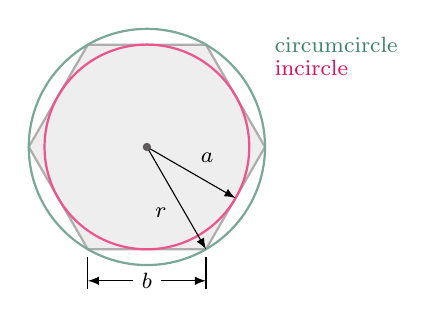
\begin{tikzpicture}
    % Indicate the boundary of the regular polygons
	\draw[thin] (-0.75,-1.4)--(-0.75,-1.8);
	\draw[thin] (0.75,-1.4)--(0.75,-1.8);
	\draw[<->] (-0.75,-1.7)--(0.75,-1.7) node[midway,fill=colorBG]{\fns{$b$}};

        \draw[thick,colorM!50,fill=colorM!10] (0:1.5cm) \foreach \x in {60,120,...,359} {
                -- (\x:1.5cm)
            }-- cycle (90:1.5cm);
	\draw [thick, colorA!70] circle (1.5cm) ;
    \draw [thick, colorB!70] circle (1.3cm) ;
	\node[colorA,align=left,anchor=west] at (1.5,1.3) {\fns{circumcircle}};
	\node[colorB,align=left,anchor=west] at (1.5,1.0) {\fns{incircle}};

	\draw[->] (0,0)--(330:1.3) node[midway,above right]{\fns{$a$}};
	\draw[->] (0,0)--(300:1.5) node[midway,below left]{\fns{$r$}};
	\fill[colorM] circle (1.5pt);
\end{tikzpicture}

Depending on the given parameter, solving for the area of the regular polygon needs a different equation.
\begin{align*}
	A &= \frac14nb^2\cot\frac{\pi}{n} \\
	A &= \frac12nr^2\sin\frac{2\pi}{n} \\
	A &= na^2\tan\frac{\pi}{n}
\end{align*}

}



\bsubgroup{Regular Polygons}
\begin{questions}

\question
How many sides has a polygon if each interior angle is 165 degrees.
\choice {32}
        {24}
        {42}
        {28}
        {b}
\Sol{
	\begin{align*}
		\theta &= \frac{180\degg(n-2)}{n} \\
		165\degg &= \frac{180\degg(n-2)}{n} \\
		n &= 24
	\end{align*}
}
        
\question
What is the number of the sides of the polygon if the sum of the measures of the angles of a convex polygon is 900?
\choice	{7}				
		{9}				
		{6}
		{8}
		{a}
\Sol{
	\begin{align*}
		\sum\theta &= 180\degg(n-2) \\
		900\degg &= 180\degg(n-2) \\
		n &= 7
	\end{align*}
}
		
\question
Which of the following regular polygons has 27 diagonals?
\choice {Nonagon}
        {Hexagon}
        {Pentagon}
        {Heptagon}
        {a}
\Sol{
	\begin{align*}
		n_d &= \frac{n}{2}(n-3) \\
		27 &= \frac{n}{2}(n-3) \\
		n &= 9
	\end{align*}
}
        
\question
Find the area of a regular pentagon whose apothem is 17.2 cm.
\choice {1075}
        {1010}
        {1142}
        {1067}
        {a}
\Sol{
	\begin{align*}
		A 	&= na^2\tan\frac{\pi}{n} \\
			&= 5(17.2)^2\tan\frac{180\degg}{5} \\
			&= 1074.7
	\end{align*}
}

\question
Find the area of a regular hexagon inscribed in a circle of radius 1
\choice	{2.698}			
		{2.598}			
		{3.698}
		{3.598}
		{b}
\Sol{
	\begin{align*}
		A 	&= \frac12nr^2\sin\frac{2\pi}{n} \\
			&= \frac12(6)(1)^2\sin\frac{360\degg}{6} \\
			&= 2.598
	\end{align*}
}

\subgroup{Plane Geometric Figures}
\Discussion{
Rectangle
\begin{align*}
	A &= ab \\
	P &= 2(a+b)
\end{align*}

Square
\begin{align*}
	A &= a^2 \\
	P &= 4a
\end{align*}

Parallelogram
\begin{align*}
	A &= bh \\
	  &= ab\sin\theta \\
	  &= \frac12d_1d_2\sin\beta \\
	P &= 2(a+b)
\end{align*}

Rhombus
\begin{align*}
	A &= ah \\
	  &= a^2\sin\theta \\
	  &= \frac12 d_1d_2 \\
	P &= 4a
\end{align*}

Trapezoid
\begin{align*}
	A &= \frac12(a+b)h
\end{align*}

Cyclic Quadrilaterals \\
- in cyclic quadrilaterals, the opposite angles are supplementary angles.
\begin{align*}
	A &= \sqrt{(s-a)(s-b)(s-c)(s-d)} \\
	s &= \frac12(a+b+c+d)
\end{align*}

Ellipse
\begin{align*}
	A &= \pi{a}{b} \\
	P &= 2\pi\sqrt{\frac{a^2+b^2}{2}}
\end{align*}

Parabola
\begin{align*}
	A = \frac23bh
\end{align*}

Spandrel
\begin{align*}
	A &= \frac13bh
\end{align*}
}

\question
A goat is tied to a corner of a 30 ft by 35 ft building. If the rope is 40 ft long and the goat can reach 1 ft farther that the rope length, what is the maximum area the goat can cover?
\choice {4084.07}
        {4840.07}
        {4804.07}
        {8044.07}
        {a}
        
\question 
An isosceles trapezoid has two base angles of 45 deg and its bases are 6 and 10. Find its area.
\choice {16}
        {10}
        {18}
        {24}
        {a}
\Sol{$2\tan45\degg\br{\frac{6+10}{2}} = 16$}
        
% \question
% A rhombus is formed by two radii and two chords of a circle of diameter 20 units. What is the area of the rhombus?
% \choice {56.78}
%         {86.60}
%         {45.76}
%         {221.70}
%         {b}

\question
The length of a side of a rhombus is 5 cm. If its shorter diagonal is of length 6 cm, what is the area of the rhombus?
\choice	{15 cm$^2$}		
		{25 cm$^2$}		
		{24 cm$^2$}
		{30 cm$^2$}
		{c}
\Sol{$5^2=3^2+\br{\frac{d_1}{2}}^2$; $d_1 = 8$; $A = \frac12(6)(8) = 24$}

\question
The perimeter of a circular sector whose central angle is 60 degrees is 14 ft. Find the radius of the circle?
\choice	{5.2 ft}			
		{4.6 ft}			
		{5.0 ft}
		{4.8 ft}
		{b}
\Sol{$P = 2r+s = 2r+r\theta^r$; $14 = 2r+r\br{\frac\pi3}$}

% \question
% The perimeter of a sector is 8 cm and its angle is 2 radians, what is the area of the sector in cm$^2$?
% \choice	{4}			
% 		{$4 \pi$}		
% 		{8}
% 		{$8 \pi$}
% 		{a}

\subgroup{Solid Geometry}
\Discussion{Polyhedrons - solid figures with flat faces

Prisms - a solid shape with a polygon as its base and is bounded by plane faces. A prism is identified by the shape of its base.

Lateral faces - all the faces other than the top and bottom faces.
\begin{align*}
	V &= A_bh \\
	A_L &= Ph
\intertext{Oblique Prism}
	V &= A_bh_{\perp} \tag{Cavalieri's Theorem} \\
	V &= A_\perp h
\intertext{Cylinders (Non-Polyhedrons)}
	V &= A_bh = \pi{r^2}h \\
	A_L &= Ch = 2\pi{r}h
\intertext{Pyramid}
	V &= \frac13A_bh \\
	A &= \text{sum of all the faces}
\intertext{Cone}
	V &= \frac13A_bh = \frac13\pi{r^2}h \\
	A &= \pi{r}L
\intertext{Frustrum}
	V &= \frac13h\br{A_1+A_2+\sqrt{A_1A_2}}
\intertext{Sphere}
	V &= \frac43\pi{r^3} \\
	A &= 4\pi{r^2}
\intertext{Spherical Wedge and Lune}
	V &= \frac43\pi{r^3} \br{\frac{\theta}{360\degg}} \\
	A &= 4\pi{r^2} \br{\frac{\theta}{360\degg}}
\intertext{Spherical Segment and Zone}
	V_\text{segment} &= \frac{\pi{h^2}}{3}(3r-h) \\
	A_\text{zone} &= 2\pi{r}h
\intertext{Spherical Cone and Pyramid}
	V_\text{s.cone} &= \frac23\pi{r^2}h \\
	V_\text{s.pyramid} &= \frac{\pi{r^3}E}{540} \\
	E &= \sum\text{angles}-(n-2)180\degg
\intertext{Torus}
	V &= \pi{r^2}(2\pi{R}) = 2\pi^2Rr^2 \\
	A &= 2\pi{r}(2\pi{R}) = 4\pi^2Rr
\intertext{Ellipsoid}
	V &= \frac43\pi{abc} \\
	V &= \frac43\pi{a^2b} \tag{oblate spheroid} \\
	V &= \frac43\pi{ab^2} \tag{prolate spheroid}
\intertext{Paraboloid}
	V &= \frac12V_c = \frac12\pi{r^2h} \\
	V &= \frac12\pi(R^2+r^2)h \tag{two bases}
\end{align*}
}

\question
The lateral area of a right prism is 162 sq.m. and the base is a rectangle 3 by 6 m. Find the altitude of the prism.
\choice {9 m}
        {8 m}
        {10 m}
        {7 m}
        {a}
\Sol{
	\begin{align*}
		A_L &= 2lh+2wh \\
			&= 2h(l+w) \\
		h 	&= \frac{162}{2(3+6)} \\
			&= 9
	\end{align*}
}
        
\question
Find the volume of a rectangular square pyramid if each edge of the base measures 10 in and the slant height of the pyramid measures 13 in.
\choice {400}
        {100}
        {200}
        {500}
        {a}
\Sol{To get the height of the pyramid, use pythagorean theorem $h = \sqrt{13^2+5^2} = 12$
\begin{align*}
	V &= \frac13A_bh \\
		&= \frac13(10)^2(12) \\
		&= 400
\end{align*}
}

\question
A large 15 m diameter cylindrical tank sits on the ground is to be painted. If one liter of paint covers 10 m$^2$, how many liters are required if it is 10 m high? (include the top)
\choice	{65}			
		{42}			
		{58}
		{49}
		{a}
\Sol{
	\begin{align*}
		A 	&= A_b+A_L \\
			&= \pi r^2 + 2\pi rh \\
		V_\text{paint} &= A\br{\frac{1\un{li}}{10\un{m^2}}} \\
			&= \bbrk{\pi(7.5)^2+2\pi(7.5)(10)}\br{\frac{1\un{li}}{10\un{m^2}}} \\
			&= 64.79
	\end{align*}
}


\question
A hemispherical bowl of radius 10 cm is filled with water to depth of 5 cm. Find the volume of the water.
\choice	{625$\pi$/3 cu.cm}			
		{625$\pi$ cu.cm}	
		{562$\pi$/3 cu.cm}
		{562$\pi$ cu.cm}
		{a}
\Sol{$V_\text{segment} = \frac{\pi{h^2}}{3}(3r-h)$ \\
\begin{center}
	\begin{tabular}{cl}
		\toprule
		0 	& 0 \\
		10 	& $\pi(10)^2$ \\
		20 	& 0 \\
		\bottomrule
	\end{tabular}
\end{center}
Save $A$, $B$, and $C$ to the corresponding memory. Then, $\int_0^5 \br{A+Bx+Cx^2} \,dx$ \\
Or This can also be solved using integration.
\begin{align*}
	V_\text{segment} &= \int_a^b \pi{y^2}\,dx \\
		&= \int_5^{10} \pi\br{\sqrt{10^2-x^2}}^2\,dx \\
		&= \int_5^{10} \pi\br{10^2-x^2}\,dx 
\end{align*}
}
\question
The volume of water in a hemisphere having a radius of 2 m is 2.05 m$^2$. Find the height of the water.
\choice	{0.602}			
		{0.782}			
		{0.498}
		{0.865}
		{a}
\Sol{Trial and Error methods
\begin{center}
	\begin{tabular}{cl}
		\toprule
		0 	& 0 \\
		2 	& $\pi(2)^2$ \\
		4 	& 0 \\
		\bottomrule
	\end{tabular}
\end{center}
Save $A$, $B$, and $C$ to the corresponding memory. Then, $\int_0^{0.602} \br{A+Bx+Cx^2} \,dx$
}

\question
The frustum of a regular triangular pyramid has equilateral triangles of its base measuring 3 m and 9 m respectively. If the bases are 8 m apart, determine its volume.
\choice {135}
        {243}
        {123}
        {175}
        {a}
\Sol{$V = \frac13h\br{A_1+A_2+\sqrt{A_1A_2}}$ \\
Or use your calculator M-3-3
\begin{center}
	\begin{tabular}{cl}
		\toprule
		0 & $(0.5)(3)^2\sin{60\degg}$ \\
		4 & $(0.5)\brk{(3+9)/2}^2\sin{60\degg}$ \\
		8 & $(0.5)(9)^2\sin{60\degg}$ \\
		\bottomrule
	\end{tabular}
\end{center}
Save $A$, $B$, and $C$ to the corresponding memory. Then, $\int_0^8 \br{A+Bx+Cx^2} \,dx$
}

\question
What is the area of a lune whose angle is 80 degrees on a sphere of radius 60 cm?
\choice	{2300$\pi$ sq.cm}		
		{3200$\pi$ sq.cm}		
		{4200$\pi$ sq.cm}
		{2400$\pi$ sq.cm}
		{b}
\Sol{
	\begin{align*}
		A_\text{lune} &= 4\pi{r}^2 \br{\frac{80}{360}} \\
			&= 3200\pi
	\end{align*}
}

\question
The volume of a spherical segment with the two bases equal to 159$\pi$. If the radii of the bases are 4 m and 5 m respectively, find the value of the altitude $h$.
\choice	{4 m}			
		{6 m}			
		{5 m}
		{7 m}
		{b}
\Sol{$V = \frac16\pi h(3a^2+3b^2+h^2)$}

\question
A spherical wooden ball is 15 cm in diameter sinks to a depth of 12 cm in a certain liquid. Determine the area exposed above the liquid.
\choice {141.37}
        {174.56}
        {235.75}
        {245.76}
        {a}
\Sol{$A_\text{zone} = 2\pi{rh} = 2\pi(7.5)(15-12) = 45\pi$}

\question
A tank in a shape of a paraboloid is filled with water of a height of 5 m and the radius of the circular section at the water surface is 3 m, Determine the volume of water inside the tank in liters.
\choice {70,\,685 li.}
        {54,\,876 li.}
        {45,\,987 li.}
        {87,\,098 li.}
        {a}
\Sol{$V = \frac12\pi{r^2h} = \frac12\pi(3)^2(5)\br{\frac{1000\un{li}}{1\un{m^3}}} = 70,685\un{li}$}

\question
A wedge is cut from a cylinder of radius 3 cm by two planes one perpendicular to the axis of cylinder and the other passing through the diameter of the section made by the first plane and inclined to this plane at an angle of 45 degrees, Find the volume of the wedge. 
\Sol{
	\begin{tabular}{cl}
		\toprule
		0 	& 0 \\
		3 	& $\frac12(3)(3)$ \\
		6 	& 0 \\
		\bottomrule
	\end{tabular} 
	$\int_0^6 \br{A+Bx+Cx^2} \,dx$
}

\Discussion{A \textbf{platonic solid} is a polyhedron all of whose faces are regular polygons. \\
Tetrahedron - 4 sides (triangle) \\
Hexahedron - 6 sides (cube) \\
Octahedron - 8 sides (triangle) \\
Dodecahedron - 12 sides (pentagon) \\
Icosahedron - 20 sides (triangle)
}

\question
Determine the total surface area of an icosahedron if the length of each edge is 10 cm.
\choice {866}
        {453}
        {203}
        {243}
        {a}
\Sol{$A = 20\brk{\frac12(10)^2\sin60\degg} = 866.03$}


\subgroup{Similar Figures}
\Discussion{
	\begin{align*}
		\frac{h_2}{h_1} &= \frac{x_2}{x_1} \\
		\frac{A_2}{A_1} &= \br{\frac{x_2}{x_1}}^2 \\
		\frac{V_2}{V_1} &= \br{\frac{x_2}{x_1}}^3 \\
	\end{align*}
}
\question
What is the percent increase in area achieved for a sphere whose diameter increases from 3 cm to 4 cm? 
\choice {78\%}
        {82\%}
        {70\%}
        {90\%}
        {a}
\Sol{
	\begin{align*}
		\text{\% increase} &= \br{\frac{A_2}{A_1}-1}100\% \\
		&= \brk{\br{\frac{d_2}{d_1}}^2-1}100\% \\
		&= \brk{\br{\frac{4}{3}}^2-1}100\% \\
		&= 77.78\%
	\end{align*}
}
\question
If the edge of the cube is increased by 20\%. Find the percentage increase in volume?
\choice {72.8\%}
        {76.3\%}
        {83.2\%}
        {63.3\%}
        {a}
\Sol{
	\begin{align*}
		\text{\% increase} &= \brk{\br{\frac{120}{100}}^3-1}100\% \\
		&= 72.8\%
	\end{align*}
}       

\subgroup{Miscellaneous Problem}

\question
Two 20 cm diameter circles are placed so that the circumference of each just touches the center of the other. What is the area common to each other?
\choice {$121.4\un{cm^2}$}
        {$123\un{cm^2}$}
        {$102.7\un{cm^2}$}
        {$145\un{cm^2}$}
        {b}
\Sol{
	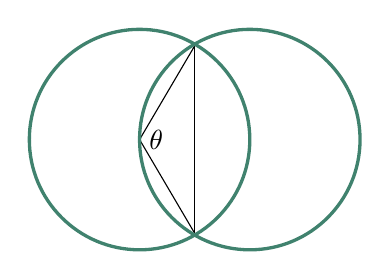
\begin{tikzpicture}[scale=0.7]
		\draw (0,1.7)--(0,-1.7);
		\draw (-1,0)--(0,1.7);
		\draw (-1,0)--(0,-1.7);
		\node[right] at (-1,0){$\theta$};
		\draw[very thick,colorA] (-1,0) circle (2);
		\draw[very thick,colorA] (1,0) circle (2);
	\end{tikzpicture}
	%
	\begin{align*}
		\cos\frac\theta2 &= \frac{5}{10} \\
		\theta &= 120 \\
		A &= 2A_\text{segment} \\
		  &= 2\brk{\pi{r^2}\frac{\theta}{360\degg}-\frac12r^2\sin\theta} \\
		  &= 2\brk{\pi(10)^2\frac{120\degg}{360\degg}-\frac12{10}^2\sin120\degg} \\
	\end{align*}
}
		
% \question
% In a circle with diameter of 10 m, a regular five-pointed star touching its circumference is inscribed. Calculate the area that is not covered by the star.
% \choice {50.48}
%         {45.12}
%         {55.46}
%         {47.82}
%         {}

\end{questions}
\END{}

\ShowHideAns



}
\end{document}

